\documentclass[11pt,reqno,final]{amsart}

\pdfcompresslevel=0
\pdfobjcompresslevel=0

\usepackage[dvipsnames]{xcolor}% adds colors
\usepackage{amsmath, amsthm}% {amsfonts, amssymb}

% New Characters
\usepackage[latin1]{inputenc}%
\usepackage[T1]{fontenc}

\usepackage{MnSymbol}
\usepackage[normalem]{ulem}% underlining

\usepackage[theoremfont, largesc]{newpxtext} % different text,math font
\usepackage{newpxmath}

\makeatletter
\DeclareMathRadical{\sqrtsign}{symbols}{112}{largesymbols}{112}
% \let\sqrt=\undefined
% \DeclareRobustCommand\sqrt{\@ifnextchar[\@sqrt{\mathpalette\@x@sqrt}]}
% \def\@x@sqrt#1#2{%
%  \setbox\z@\hbox{$\m@th#1\sqrtsign{\mkern1mu #2}$}
%  \mkern3mu\box\z@}
\makeatother




% Page Typesetting
\usepackage[final]{microtype}
\usepackage{relsize}
\usepackage[margin=1in]{geometry}
\usepackage{framed}
\usepackage{tikz}

\usepackage{setspace}
\onehalfspacing

\usepackage{hyperref}
\hypersetup{
  final,
  pdftitle={Math 135 - Derivative Rules 1},
  pdfauthor={Bonventre}, 
  linktoc=page,
  pagebackref,
  colorlinks=true,
  citecolor=PineGreen,
  linkcolor=PineGreen,
  linkbordercolor=PineGreen,
}


% Internal References

\usepackage[inline,shortlabels]{enumitem}

% \numberwithin{equation}{section} 
\numberwithin{figure}{section}

\usepackage[nameinlink,capitalise,noabbrev]{cleveref}

\crefname{equation}{}{} % get \cref to behave as \eqref

% \theoremstyle{plain} % bold name, italic text
\newtheorem{theorem}[equation]{Theorem}%
\newtheorem*{theorem*}{Theorem}%
\newtheorem{lemma}[equation]{Lemma}%
\newtheorem{proposition}[equation]{Proposition}%
\newtheorem{corollary}[equation]{Corollary}%
\newtheorem{conjecture}[equation]{Conjecture}%
\newtheorem*{conjecture*}{Conjecture}%
\newtheorem{claim}[equation]{Claim}%
\newtheorem{question}{Question}

\theoremstyle{definition} % bold name, plain text
\newtheorem{definition}[equation]{Definition}%
\newtheorem*{definition*}{Definition}%
\newtheorem{example}[equation]{Example}%
\newtheorem*{example*}{Example}%
\newtheorem{remark}[equation]{Remark}%
\newtheorem{notation}[equation]{Notation}%
\newtheorem{convention}[equation]{Convention}%
\newtheorem{assumption}[equation]{Assumption}%
\newtheorem{exercise}[question]{Exercise}

% ---------- macros
\newcommand{\set}[1]{\left\{#1\right\}}%
\newcommand{\sets}[2]{\left\{ #1 \;|\; #2\right\}}%
\newcommand{\longto}{\longrightarrow}%
\newcommand{\into}{\hookrightarrow}%
\newcommand{\onto}{\twoheadrightarrow}%

\usepackage{harpoon}
\newcommand{\vect}[1]{\text{\overrightharp{\ensuremath{#1}}}}

\newcommand{\del}{\partial}%

\newcommand{\ki}{\chi}
\newcommand{\ksi}{\xi}
\newcommand{\Ksi}{\Xi}

\newcommand{\dlim}{\displaystyle\lim}

% %%%%%%%%%%%%%%%%%%%%%%%%%%%%%%%%%%%%%%%%%%%%%%%%%%%%%%%%%%%%%%%%%%%%%%%%%%%%%%%%%%%%%%%%%%%%%%%%%%%%

\begin{document}


\begin{center}
        \textbf{\Large Math 135, Calculus 1, Fall 2020}\\[10pt]
        {\large 10-12: Derivative Rules 1}
\end{center}

\thispagestyle{empty}


\renewcommand{\thesection}{\Alph{section}}

% \vspace{-1pt}

Last week, we introduced the \textbf{derivative function} $f'(x)$ of a function $f(x)$, whose evaluation $f'(a)$ at the point $x=a$ is give by:
\begin{itemize}
\item the slope of the tangent line at $x=a$
\item the instantaneous velocity at time $x = a$
\end{itemize}

In general, the rule of the derivative function $f'(x)$ can be computed as the limit
\[
        f'(x) = \dlim_{h \to x} \dfrac{f(x+h) - f(x)}{h}
\]
where the numerator is (and remains) a function of $x$.
However, this \textbf{limit definition of the derivative} can be cumbersome.
If only there were some \textbf{rules} or \textbf{patterns} we could find, that would help us not need to go through the elaborate limit calculations.

We saw the first of these last Friday: the derivative when $f(x) = mx + b$ is a line is just the \textit{constant function} $f'(x) = m$ at the slope of the line.
This was proved using the limit definition of the derivative, but now we never need to use it again for a line.

\section{``There's got to be a better way!''}

The following formulas can all be computed using the limit definition of the derivative.
However, they are \textbf{general}, and can then be used when computing the derivative of many different functions.

\begin{itemize}\itemsep+15pt
\item \textbf{Constant Rule:} $\dfrac{d}{dx}(c) = 0$
\item \textbf{Power Rule:} $\dfrac{d}{dx}(x^n) = nx^{n-1}$ for \textbf{any} real number $n$.
\item \textbf{Constant Multiples:} $\dfrac{d}{dx}\big(c \cdot f(x)\big) = c \cdot f'(x)$ for any constant $c$
\item \textbf{Sums and Differences:} $\dfrac{d}{dx}\big( f(x) \pm g(x) \big) = f'(x) \pm g'(x)$
\item \textbf{Exponential Functions:} $\dfrac{d}{dx}(b^x) = \ln b \cdot b^x$, so in particular $\dfrac{d}{dx}(e^x) = e^x$.
\end{itemize}

\begin{exercise}
        Verify the Power Rule when $n = 3$; that is, use the limit definition of the derivative to show that $\dfrac{d}{dx}(x^3)=3x^2$.
\end{exercise}

\newpage

\begin{exercise}
        Find each of the following derivatives using the power rule:\\
        \begin{enumerate*}[(a)]
        \item $\dfrac{d}{dx}(x^{15})$ \qquad \qquad $ $
        \item $\dfrac{d}{dx}\left( \dfrac{1}{x^4} \right)$ \qquad \qquad $ $
        \item $\dfrac{d}{dx}(\sqrt{x})$ \qquad \qquad
        \item $\dfrac{d}{dx}(x^\pi)$\\
        \end{enumerate*}
\end{exercise}

$ $\\[10pt]

\begin{exercise}
        Find $g'(x)$ if $g(x) = 6\sqrt{x} - \dfrac{3}{x^3} + 5e^x - \pi^4$.
        \vfill
\end{exercise}

\begin{exercise}
        If $p(x) = 4 \sqrt[3]{x} + \dfrac{2}{3} x - \dfrac{8}{x}$,
        find the equation of the tangent line to $p$ at the point $x=8$.
        \vfill
\end{exercise}

\begin{exercise}
        Use the limit definition of the derivative to verify that $\dfrac{d}{dx}(e^x) = e^x$.
        You may use the following: $\dlim_{x \to 0}\dfrac{e^x-1}{x} = 0$.
        \vfill
\end{exercise}

\newpage

\begin{exercise}
        If the graph of $g(t)$ is a parabola, what type of graph will $g'(t)$ be? Explain.
        \vfill
\end{exercise}
        
\begin{exercise}
        If $z = e^t + t^e$, find $\dfrac{dz}{dt}$.
        \vfill
        \vfill
\end{exercise}

\begin{exercise}
        The graph belows shows three functions: $f(x)$, $g(x)$, and $h(x)$.
        If $f'(x) = g(x)$ and $g'(x) = h(x)$, identify that graph that represents each function. Explain.\\
        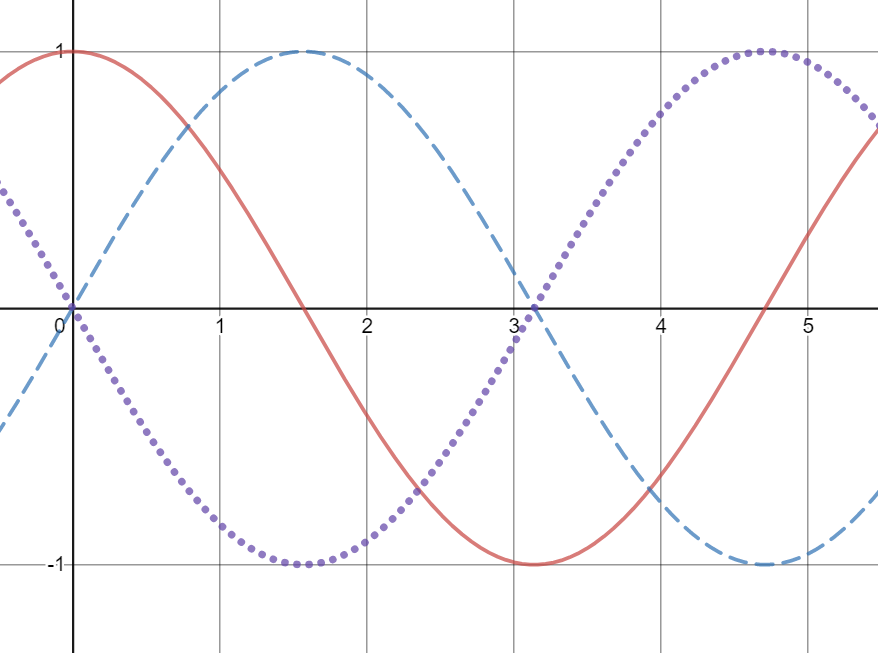
\includegraphics[width=3in]{10-12P_sins.png}
        \vfill
\end{exercise}

\end{document}
